\begin{frame}{encapsulation options [incomplete]}
\small
\begin{tabular}{l||p{4cm}|p{4cm}|p{2cm}}
left in above       & TCP/UDP/higher layers & IP & link-layer \\ \hline \hline
above TCP/UDP       & HTTP proxy, DNS over HTTP(S) & --- & --- \\ \hline
TCP/UDP             & SOCKS, HTTP CONNECT, SSH conn forwarding, TLS & --- & --- \\\hline
IP                  & OpenVPN, WireGuard & GRE, IPsec & MPLS \\\hline
link-layer          & OpenVPN, \ldots & ? & VLAN, MPLS \\\hline
\end{tabular}
\end{frame}

\begin{frame}<2>[label=encapChanges]{encapsulating w/o app changes}
\begin{itemize}
\item generally: easier to do for lower layers
\vspace{.5cm}
\item link-layer
    \begin{itemize}
    \item \myemph<2>{``virtual'' (probably Ethernet) device}
    \item \myemph<2>{sends/receives from `tunnel'}
    \end{itemize}
\item IP
    \begin{itemize}
    \item \myemph<3>{``virtual'' IP link}
    \item \myemph<3>{destination routing table can go to}
    \end{itemize}
\item UDP/TCP
    \begin{itemize}
    \item \myemph<4>{replace socket API}
    \item \myemph<5>{convince application to connect to different IP address?}
    \item \myemph<6>{use virtual IP link + implement one end of TCP/UDP}
    \end{itemize}
\end{itemize}
\end{frame}

\againframe<2>{encapChanges}

\begin{frame}[fragile]{Linux tap devices}
\begin{Verbatim}[fontsize=\fontsize{10}{11}]
# create virtual ethernet device mydev
$ ip tuntap add dev mydev mode tap
# mark ethernet device as up
$ ip link set mydev up
$ dhclient mydev # or other commands to use/config device
\end{Verbatim}
(dhclient is a DHCP client) \\
---
\begin{Verbatim}[fontsize=\fontsize{10}{11}]
int opentap(const char * name) {
    ... /* setup code, not shown*/
}
...
int fd = opentap("mydev");
...
write(fd, ethernetPacket, packetSize)
/* and (probably in separate threads) */
read(fd, buffer, SIZE); processEthernetPacket(buffer);
\end{Verbatim}
\end{frame}

\againframe<3>{encapChanges}

\begin{frame}[fragile]{Linux tun devices}
    \begin{itemize}
    \item same as `tap' devices, but\ldots
    \item get IP packets, not ethernet packets
    \end{itemize}
\begin{Verbatim}[fontsize=\fontsize{10}{11}]
# create virtual ethernet device mydev
$ ip tuntap add dev mydev mode tun
# setup device to be routed to, example:
$ ip address add 10.0.0.2 dev mydev
$ ip route add 10.0.0.0/24 dev mydev
$ ip -6 address add 3fff:1234::1 dev mydev
$ ip -6 route add 3fff:1234::/32 dev mydev
\end{Verbatim}
    \begin{itemize}
    \item tunneling program can then open device and read/write IP packets
    \end{itemize}
\end{frame}

\begin{frame}[fragile]{full tunnel routing table}
say 198.51.100.5 is running tunnel sever, \\
and 10.0.2.5  is gateway beyond tunnel, \\
and 203.0.113.54 is local gateway: \\
\begin{tabular}{l|l|l|l}
address & next hop & dev & priority\\ \hline
10.0.2.0/24 & --- & tunnel & normal \\
198.51.100.5/32 & 208.0.113.54 & real & high\\
(default) & 203.0.113.54 & real & normal \\
(default) & 10.0.2.5 & tunnel & high \\
\end{tabular}
\end{frame}


\begin{frame}[fragile]{split tunnel routing table}
say 198.51.100.5 is running tunnel sever, \\
and 10.0.2.5  is gateway beyond tunnel, \\
and 10.0.0.0/16, 198.51.100.0/24 are tunneled networks \\
and 203.0.113.54 is local gateway: \\
\begin{tabular}{l|l|l|l}
address & next hop & dev & priority\\ \hline
10.0.2.0/24 & --- & tunnel & normal \\
10.0.0.0/16 & 10.0.2.5& tunnel & normal \\
198.51.100.0/24 & 10.0.2.5& tunnel & normal \\
198.51.100.5/32 & 208.0.113.54 & real & high\\
(default) & 203.0.113.54 & real & normal \\
\end{tabular}
\end{frame}

\againframe<4>{encapChanges}

\begin{frame}[fragile]{`transparent' proxy (1)}
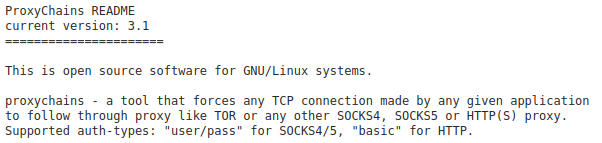
\includegraphics[width=\textwidth]{../encap/proxy-chains}
\begin{itemize}
\item configures dynamic library loader to load its library
    \begin{iteimze}
    \item \texttt{LD\_PRELOAD}
    \end{itemize}
\item with special versions of \texttt{connect}
\end{itemize}
\end{frame}

\againframe<5>{encapChanges}

\begin{frame}
    % FIXME
\end{frame}

\againframe<6>{encapChanges}

\begin{frame}
    % FIXME
\end{frame}
